\documentclass{article}
\usepackage{graphicx}
\usepackage{wrapfig}
\usepackage{filecontents}
\usepackage{siunitx}
\usepackage[table]{xcolor}
\usepackage{float}
\usepackage{hyperref}

\usepackage{color} % balíček pro obarvování textů
\usepackage{xcolor}  % zapne možnost používání barev, mj. pro \definecolor
\usepackage[total={175mm,230mm}, top=23mm, left=20mm, includefoot]{geometry}
\hypersetup{
    colorlinks,
    linkcolor={blue!50!black},
    citecolor={green!50!black},
    urlcolor={blue!80!black}
}
\definecolor{orange}{RGB}{ 251, 114, 032}
\definecolor{fialova}{RGB}{ 255, 000, 255}

\newcommand \obr[1]
{ obr. \ref{#1}}

\newcommand \tab[1]
{ tab. \ref{#1}}


% \usepackage{lmodern}
% \usepackage{amssymb,amsmath}
% \usepackage{ifxetex,ifluatex}
% \usepackage{fixltx2e} % provides \textsubscript
% \ifnum 0\ifxetex 1\fi\ifluatex 1\fi=0 % if pdftex
%   \usepackage[T1]{fontenc}
%   \usepackage[utf8]{inputenc}
% \else % if luatex or xelatex
%   \ifxetex
%     \usepackage{mathspec}
%   \else
%     \usepackage{fontspec}
%   \fi
%   \defaultfontfeatures{Ligatures=TeX,Scale=MatchLowercase}
% \fi

% \usepackage{pgfplots} % http://www.chiark.greenend.org.uk/doc/texlive-doc/latex/pgfplots/pgfplots.pdf
% \usepackage{blindtext}

% \usepackage{subfiles} % Best loaded last in the preamble

% \usepackage{bookmark}
% \usepackage{tikz}
% \usetikzlibrary{patterns}

% \usepgfplotslibrary{polar}
% \usepgfplotslibrary{external}
% \usepgfplotslibrary{fillbetween}

\begin{document}
\section*{Laboratorní cvičení č. 2 – Měření napětí - stejnosměrné a střídavé voltmetry}

\textbf{
    \begin{itemize}
        \item Autor: Tomáš Vavrinec
        \item Datum měření: 3.10.2022
    \end{itemize}
}

\subsection*{Úkoly}

\begin{enumerate}
    \item Pomocí referenčního multimetru Agilent34401A ověřte přesnost voltmetru laboratorního zdroje GWInstek GPD-3303S v rozsahu 0 až 10 V DC s krokem měření 1V. Vypočtěte absolutní a relativní chyby měření stejnosměrného napětí, korekci K a vykreslete korekční křivku, za předpokladu, že správné hodnoty napětí udává multimetr Agilent 34401A.
    \item Změřte vstupní odpor Rvst multimetru Keysight 34450A na rozsahu 10 V DC a vstupní odpor Rvst multimetru Agilent (HP) 34401A na rozsahu 1 V DC pomocí napěťového děliče. Jako zdroj ss. napětí použijte funkční generátor Siglent SDG2042X. Naměřené hodnoty porovnejte s údajem od výrobce.
    \item Změřte frekvenční charakteristiky multimetrů Keysight 34450A a Agilent 34401A pro sinusový signál z generátoru Siglent SDG 2042X s amplitudou 1,5 V v rozsahu 1 kHz až 500 kHz (zvolit minimálně 10 hodnot). Dosažené výsledky graficky zakreslete. Zhodnoťte dosažené výsledky měření na základě informací o frekvenčním rozsahu multimetrů zjištěných ze specifikace přístroje.
    \item Multimetrem Keysight 34450A změřte efektivní hodnotu výstupních signálů, jejichž zdrojem je generátor Siglent SDG 2042X:
    \begin{itemize}
        \item Obdélníkový průběh, f =1 kHz, Up-p=3 V
        \item Trojúhelníkový průběh, f =100 Hz, Up-p=5 V 
    \end{itemize}
    Průběhy signálů zakreslete do sešitu a popište.
    Ověřte výpočtem velikosti efektivních hodnot uvedených signálů, vypočtěte absolutní a relativní chybu měření (správnou hodnotou je hodnota vypočtená) a dosažené výsledky zhodnoťte.
    Určete velikost absolutních a relativních chyb údaje multimetru Keysight 34450A pro tato měření.
    \item U číslicového multimetru Agilent 34401A ve funkci stejnosměrného voltmetru s nastavením rozlišení 4digit/slow a 5digit/slow změřte na rozsahu 1V závislost činitele potlačení sériového rušení H na frekvenci fr rušivého napětí. Frekvenci volte v rozsahu fr = 45 až 55 Hz po kroku 1 Hz u rozlišení 4digit/slow a po kroku 0,5 Hz u rozlišení 5digit/slow. Hodnota napětí Uss je nulová (pro zjednodušení).
\end{enumerate}

\section*{Příprava}
Nejčastější měření v elektrotechnice je měření napětí.
Voltmetry mohou být rozděleny podle:

\begin{figure}[H]
    \scriptsize
    {
        \begin{minipage}[t]{0.24\textwidth}
            1) způsobu měření
            \begin{itemize}
                \item analogové
                \item číslicové (digitální).
            \end{itemize}
        \end{minipage}
        \hfill
        \begin{minipage}[t]{0.24\textwidth}
            2) podle druhu měřeného napětí: 
            \begin{itemize}
                \item stejnosměrné 
                \item střídavé
                \item impulsní
            \end{itemize}
        \end{minipage}
        \hfill
        \begin{minipage}[t]{0.24\textwidth}
            3) podle citlivosti
            \begin{itemize}
                \item voltmetry
                \item milivoltmetry
                \item mikrovoltmetry
                \item nanovoltmetry.
            \end{itemize}
        \end{minipage}
        \hfill
        \begin{minipage}[t]{0.24\textwidth}
            4) podle kmitočtové oblasti (střídavé voltmetry):
            \begin{itemize}
                \item nízkofrekvenční
                \item vysokofrekvenční
                \item širokopásmové
                \item selektivní (úzkopásmové)
            \end{itemize}
        \end{minipage}
    }
\end{figure}

\subsection*{Korekční křivka}
Pokud chceme zvýšit přesnost měření konkrétního přístroje můžeme k jeho měření přičítat hodnotu z korekční křivky.
Korekční křivku můžeme získat porovnáním měření s přesnějším přístrojem (etalonem) \(k = -\delta_x = X_S X_M\) kde \(X_S\) je hodnota naměřena na etalonu a \(X_M\) je hodnota naměřena na kontrolovaném přístroji.
\begin{figure}[H]
    % \centering
    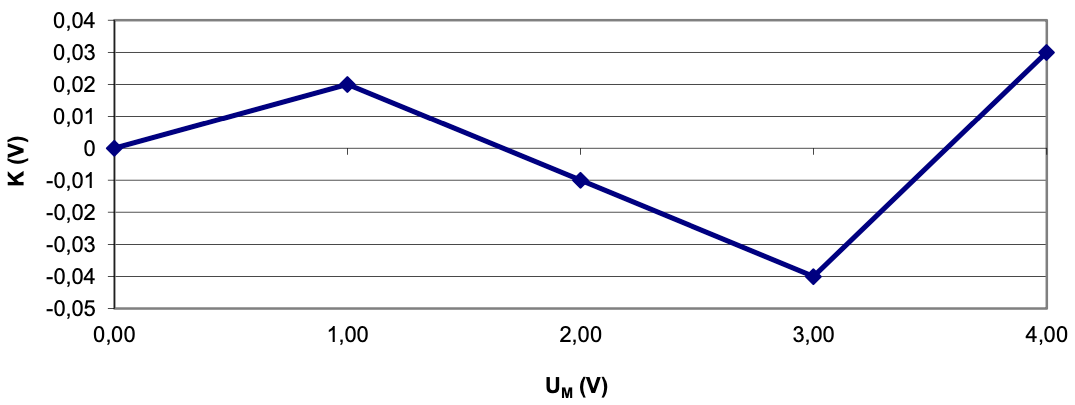
\includegraphics[width=\textwidth]{obrazky/korekcni_krivka.png}
    \caption{\label{korek_krivka}Příklad korekční křivky}
\end{figure}

\subsection*{Vstupní odpor voltmetru}
\begin{wrapfigure}{r}{0.5\textwidth}
    \vspace{-10mm}
    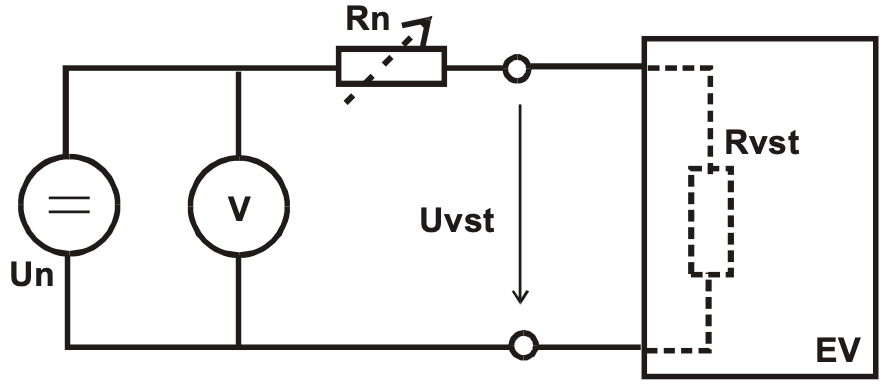
\includegraphics[width=0.5\textwidth]{obrazky/vstup_odpor.png}
    \caption{\label{vstupni_odpor}Zapojení pro měření vstupního odporu voltmetru}
\end{wrapfigure}
Vstupní odpor voltmetru je odpor, který je mezi vstupními vodiči a zemí.
Dá se jednoduše určit pomocí zdroje napětí a rezistoru se srovnatelným odporem.
\(R_{vst}=\frac{U_{vst}}{U_{n}-U_{vst}}\)

\subsection{Měření AC}
Běžný frekvenční rozsah se pohybuje od \(100\-kHz\) do \(1\-MHz\).
Jeden z parametrů AC voltmetru je způsob měření efektivní hodnoty.
Buď měřený signál usměrní, změří jeho střední hodnotu a převede ji na efektivní, tato metoda je však přesná jen pro harmonický signál (střední hodnota se násobí konstantou která souvisí s konkrétním tvarem signálu a pochopitelně se proto používá nejběžnější tvar).
Druhá možnost je signál měřit pomocí definice efektivní hodnoty, která je vypočítána takto:
\begin{equation}
    U_{efe} = \sqrt{\frac{1}{T}\int_{0}^{T}U^2(t)dt}
    \label{proud_kolektoru}
\end{equation}


% Tranzistor je typická nelineární součástka v obvodu popsatelná šesti veličinami, třemi proudy a třemi napětími vyznačenými na \obr{pracovni_bod_tranzistoru} a) (\(I_C I_B I_E U_{CE} U_{BE} U_{BC})\).
% Tyto veličiny jsou propojeny nelineárními závislostmi které lze chápat jako šestirozměrný objekt, kterým když provede dvourozměrný řez dostaneme např. výstupní charakteristiku (závislost \(I_C\) na \(U_{CE}\)
% při konstantním proudu \(I_B\)).
% \vspace{-1mm}

% Pokud tranzistory zapojíme do zapojení na \obr{pracovni_bod_tranzistoru} b) při \(U_{in} = 0\) ustálí se jeho veličiny na konkrétním bodě, tento bod označujeme \(Q\) a nazýváme ho stejnosměrný pracovní bod tranzistoru.
% Aby mohl tranzistor fungovat jako zesilovač správně je nutné aby nastavení pracovního bodu umožňovalo v oběma směry dostatečný rozkmit výstupního signálu v dostatečné míře bez přílišného zkreslení.
% Pracovní bod se proto obvykle nastavuje tak aby v ustáleném stavu platilo \(U_{out} = \frac{1}{2}V_{cc}\)

% \vspace{1mm}
% \begin{wrapfigure}{r}{0.5\textwidth}
%   % \centering
%   \vspace{-10mm}
%   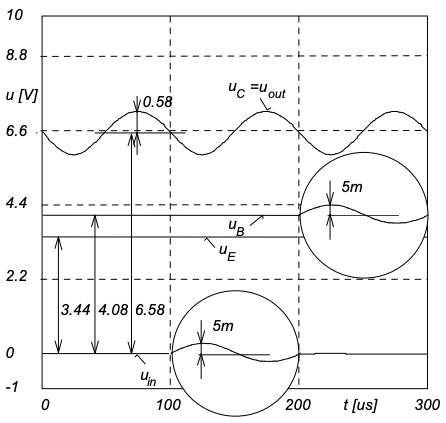
\includegraphics[width=0.5\textwidth]{vstup-baze-vystup.png}
%   \caption{\label{vstup_baze_vystup}}
% \end{wrapfigure}
% Abychom mohli na tento zesilovač přivést signál s jiným středním napětím neš jaké je na bázi tranzistoru, přípojíme vstup zesilovače na bázi skrz kapacitu \(C_1\).
% Tato kapacita musí být dostatečně velká aby se pro signál o požadované frekvenci dala považovat za zkrat.
% Na \obr{vstup_baze_vystup} je zobrazen možný procházející signál.

% Při nastavování pracovního bodu je mimo jiné nezbytné znát následující vztahy
% \newpage

% \section{Počítačové cvičení}
% \begin{figure}[H]
% 	\begin{minipage}[t]{0.45\textwidth}
%     \vspace{-5mm}
%     \begin{figure}[H]
%       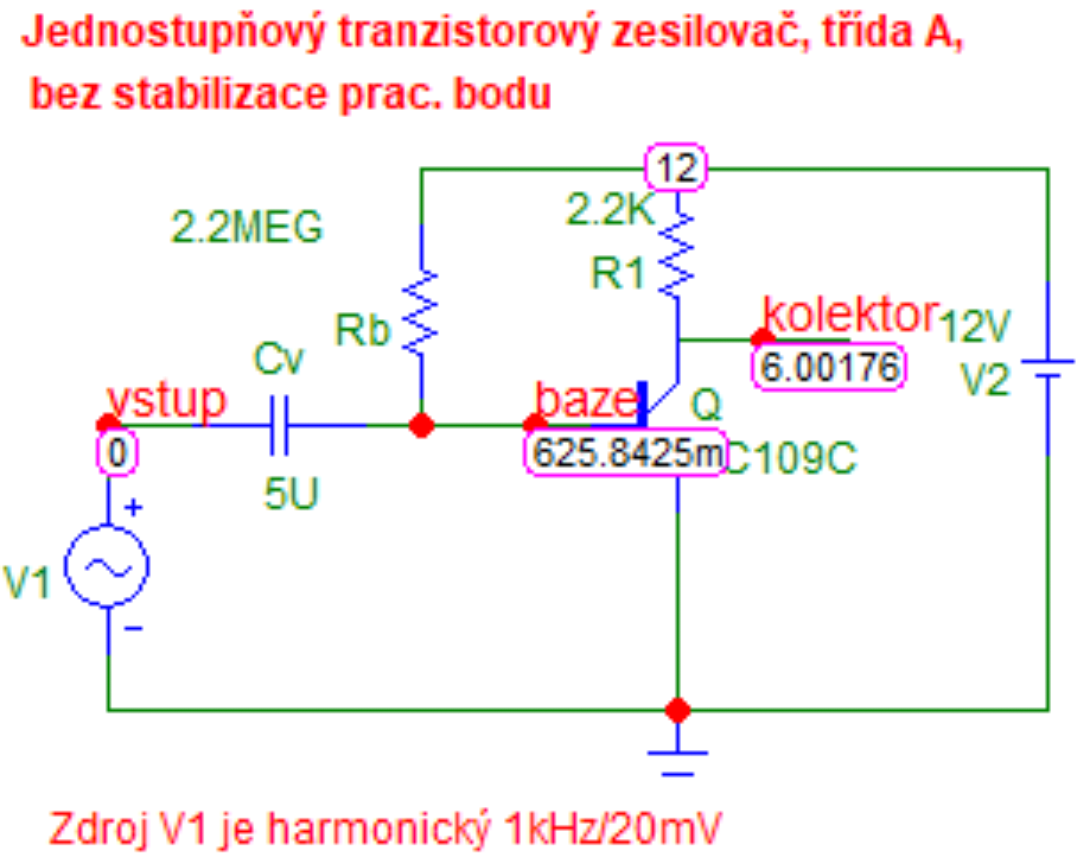
\includegraphics[width=\textwidth]{PC/BJT/prac_bod.png}
%       % \addlegendentry{test}
%       \caption{\label{prac_bod_sim_1} Stejnosměrné nastavení pracovního bodu}
%     \end{figure}
%   \end{minipage}
%   \hfill
%   \begin{minipage}[t]{0.45\textwidth}
%     \begin{figure}[H]
%       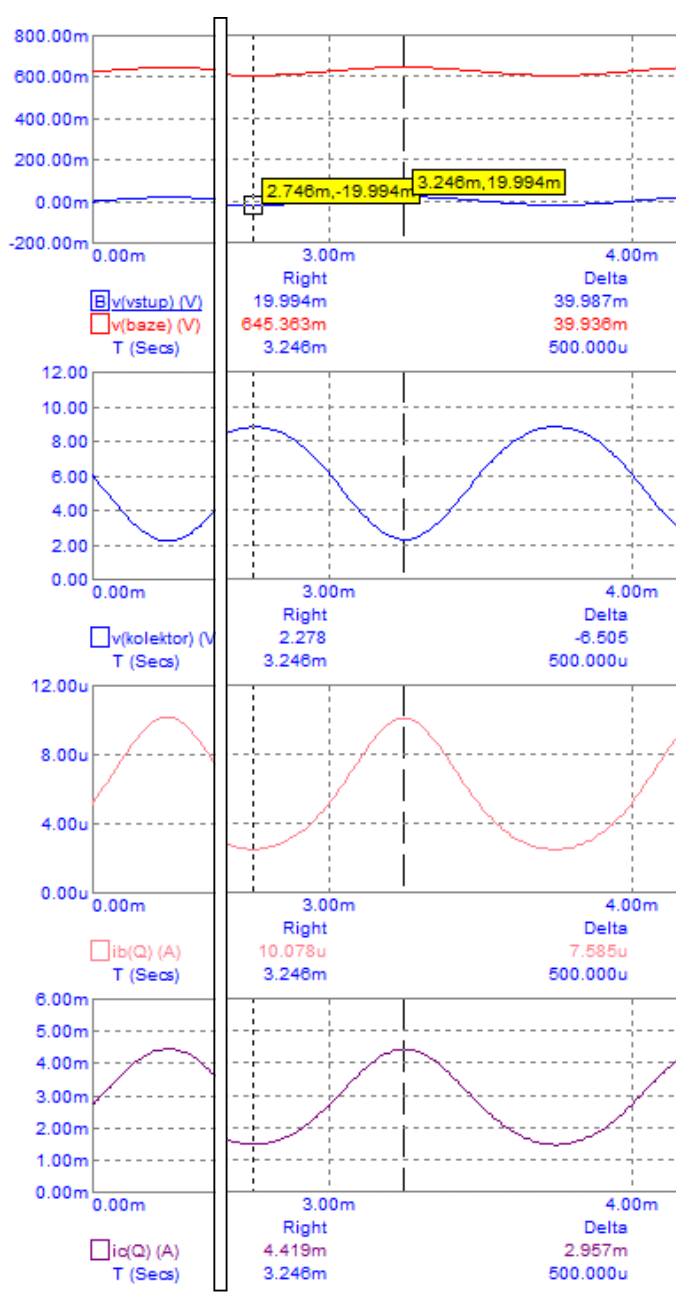
\includegraphics[width=\textwidth]{PC/BJT/sim_1.png}
%       % \addlegendentry{test}
%       \caption{\label{prac_bod_sim_1} Odezva na základní sinusoví signál}
%     \end{figure}
%   \end{minipage}
% \end{figure}

% \begin{figure}[H]
% 	\begin{minipage}[t]{0.471\textwidth}
%     \begin{figure}[H]
%       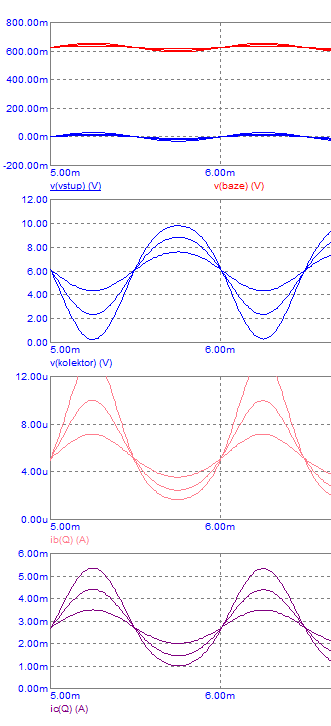
\includegraphics[width=\textwidth]{PC/BJT/Tranzient_analyza_3.png}
%       \caption{\label{prac_bod_sim_1} Sinusový průběh při změně \(U_{in}\)}
%     \end{figure}
%   \end{minipage}
%   \hfill
% 	\begin{minipage}[t]{0.4\textwidth}
%     \begin{figure}[H]
%       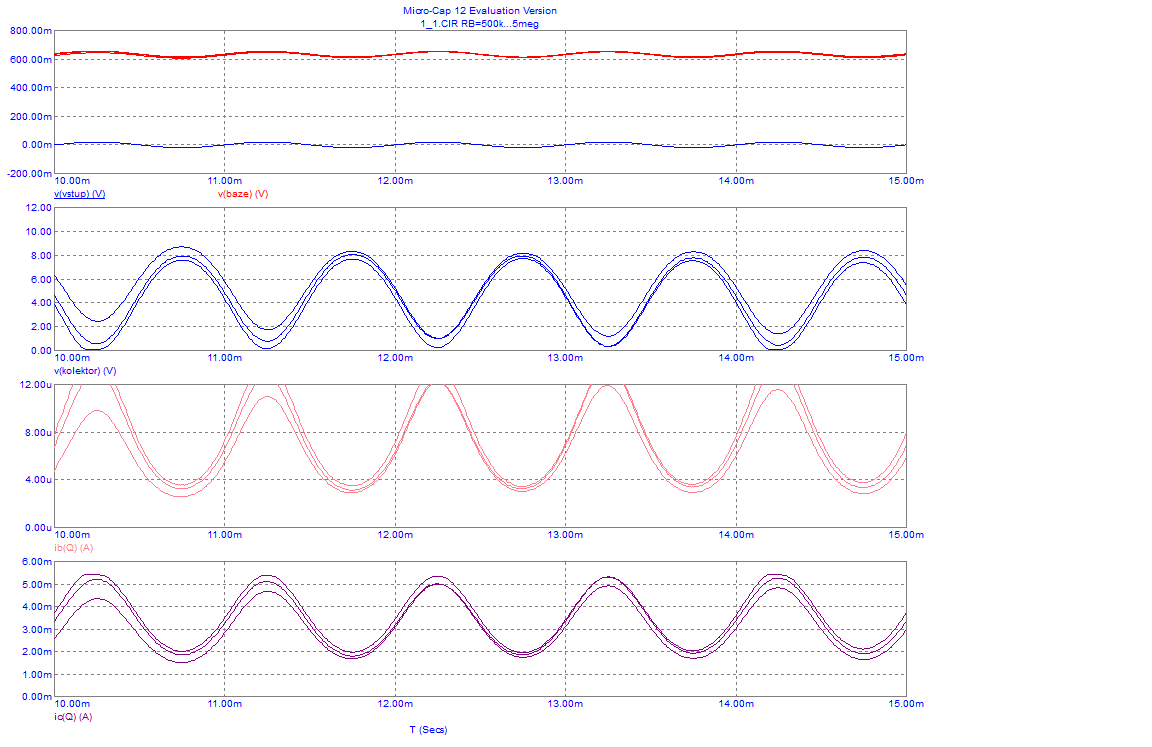
\includegraphics[width=\textwidth]{PC/BJT/Tranzient_analyza_4.png}
%       \caption{\label{prac_bod_sim_1} Sinusový průběh při změně \(R_b\)}
%     \end{figure}
%   \end{minipage}
% \end{figure}

% \hfill
% \begin{figure}[H]
%   \includegraphics[width=\textwidth]{PC/BJT/Sirka_pasma.png}
%   \caption{\label{prac_bod_sim_1} Šířka pásma při \(C_v = 5 \mu F\)}
% \end{figure}
% \begin{figure}[H]
%   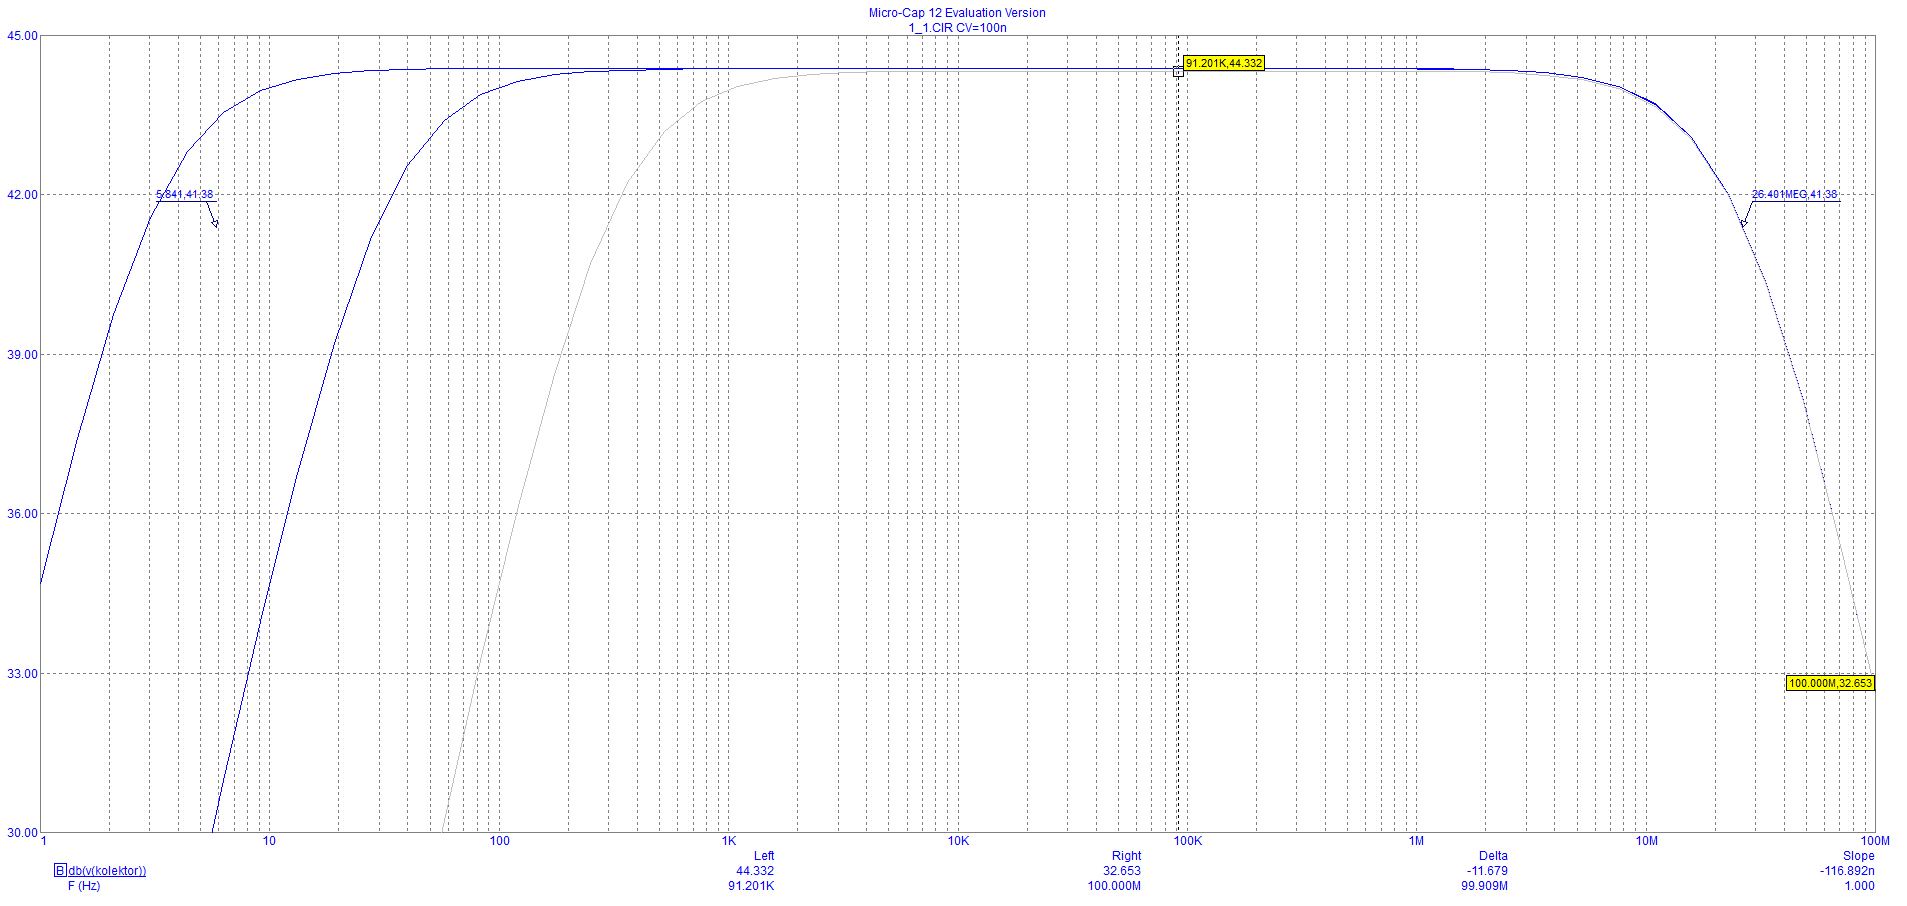
\includegraphics[width=\textwidth]{PC/BJT/Step_sirka_pasma.png}
%   \caption{\label{prac_bod_sim_1} Šířka pásma při změně \(C_v\)}
% \end{figure}

% \newpage

% \section{Laboratorní cvičení}
% % \subsections{zadání}
% % Nejprve sestavte obvod bez vazebního kondenzátoru a zdroje signálu. Změnou odporu Rb
% % nastavte ss napětí na kolektoru tranzistoru 6 V. Změřte všechna uzlová napětí a z nich dopočtěte
% % větvové proudy. Porovnejte s výsledky z NC a PC.
% % Doplňte obvod o Cv a generátor signálu. Proveďte „oživení“ zesilovače pomocí osciloskopu.
% % Zesilovač nesmíte přebudit výstupní napětí nesmí vykazovat zkreslení. Měřte při kmitočtu
% % 1 kHz. Zakreslete časové průběhy vstupního napětí, napětí na bázi a na kolektoru, včetně ss
% % posunutí. Změřte amplitudy a vypočtěte z nich střídavá zesílení.

% \begin{figure}[H]
% 	\begin{minipage}[t]{0.6\textwidth}
%     Měřili jsme s tranzistorem BC55 u kterého jsme na začátku naměřili \(\beta = 422\)
%     Nejprve jsme sestavili obvod a pomocí potenciometru jsme nastavili pracovní bod dle \tab{tab_pracovni_bod}.
%     \vspace{5mm}
%     \begin{table}[H]
%       % \centering
%       \begin{tabular}{|c|c|c|c|} 
%         \hline
%          \(U_{cc}\-[V]\) & \(U_{c}\-[V]\)  & \(R_b\-[M\Omega]\) &	\(R_c\-[K\Omega]\) \\ \hline
%          12              & 6               & 2.5                & 2.2                \\ \hline
%       \end{tabular}
%       \caption{\label{tab_pracovni_bod} Nastavení obvodu}
%     \end{table}
%   \end{minipage}
%   \hfill
% 	\begin{minipage}[t]{0.4\textwidth}
%     \begin{figure}[H]
%       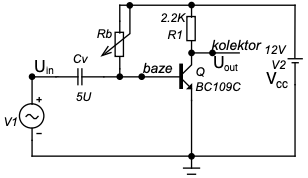
\includegraphics[width=\textwidth]{obvod-z-laborky.png}
%       \caption{\label{obvod_z_laborky}}
%     \end{figure}
%   \end{minipage}
% \end{figure}

\end{document}
